\section{Simulaiton}
\markright{Simulaiton}

\begin{figure}[H]
  \centering
  \begin{subfigure}[b]{0.48\textwidth}
    \centering
    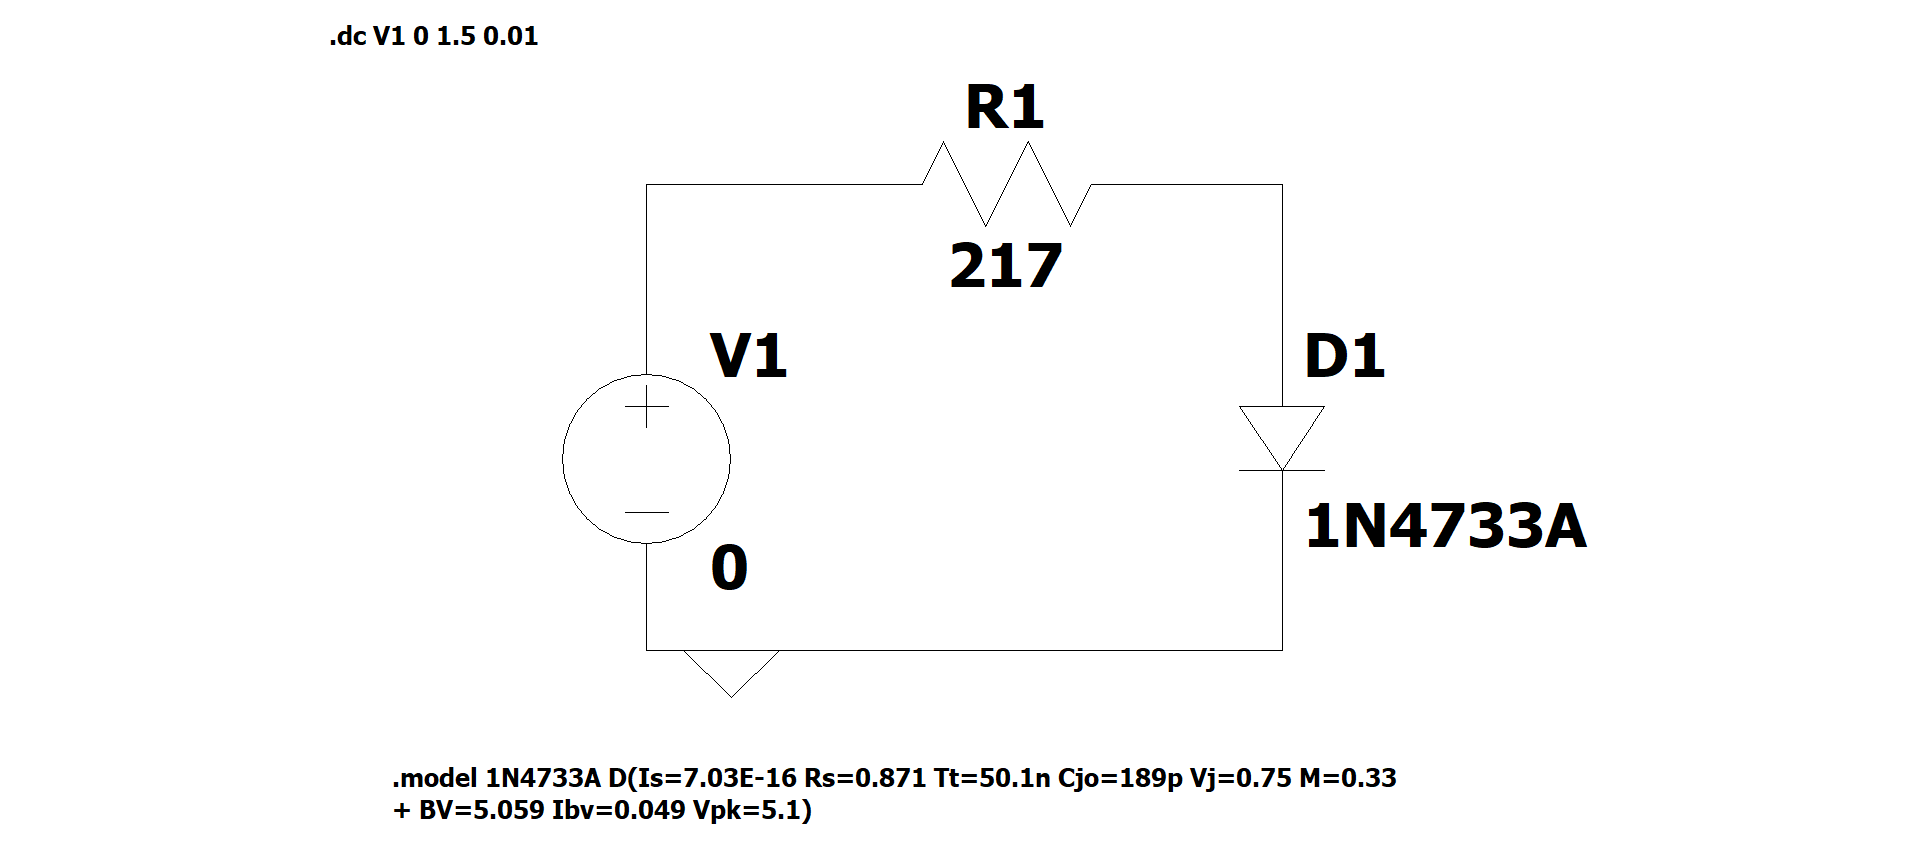
\includegraphics[width=\textwidth, height=4.5cm, keepaspectratio]{lab-06/assets/forward-schematic.png}
    \caption{Schematic}
  \end{subfigure}
  \hfill
  \begin{subfigure}[b]{0.48\textwidth}
    \centering
    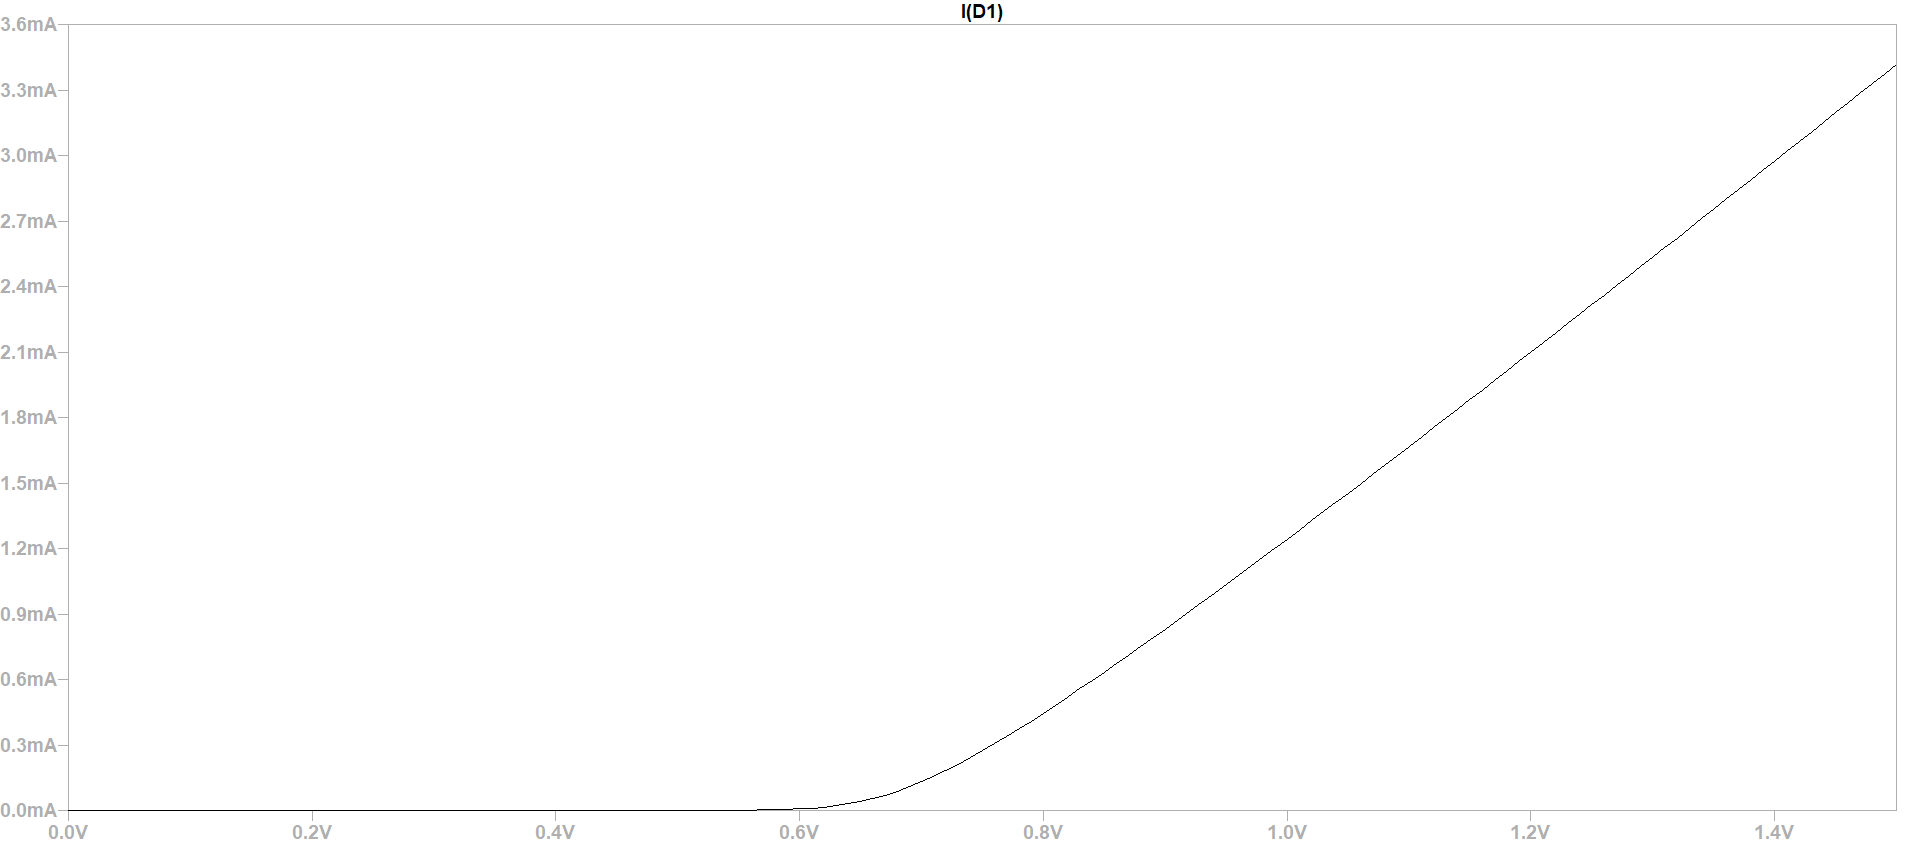
\includegraphics[width=\textwidth, height=4.5cm, keepaspectratio]{lab-06/assets/forward-graph.png}
    \caption{Output}
  \end{subfigure}
  \caption{Simulation of Forward Bias: (a) Schematic and (b) Output.}
  \label{fig:lab06_sim_forward}
\end{figure}

\begin{figure}[H]
  \centering
  \begin{subfigure}[b]{0.48\textwidth}
    \centering
    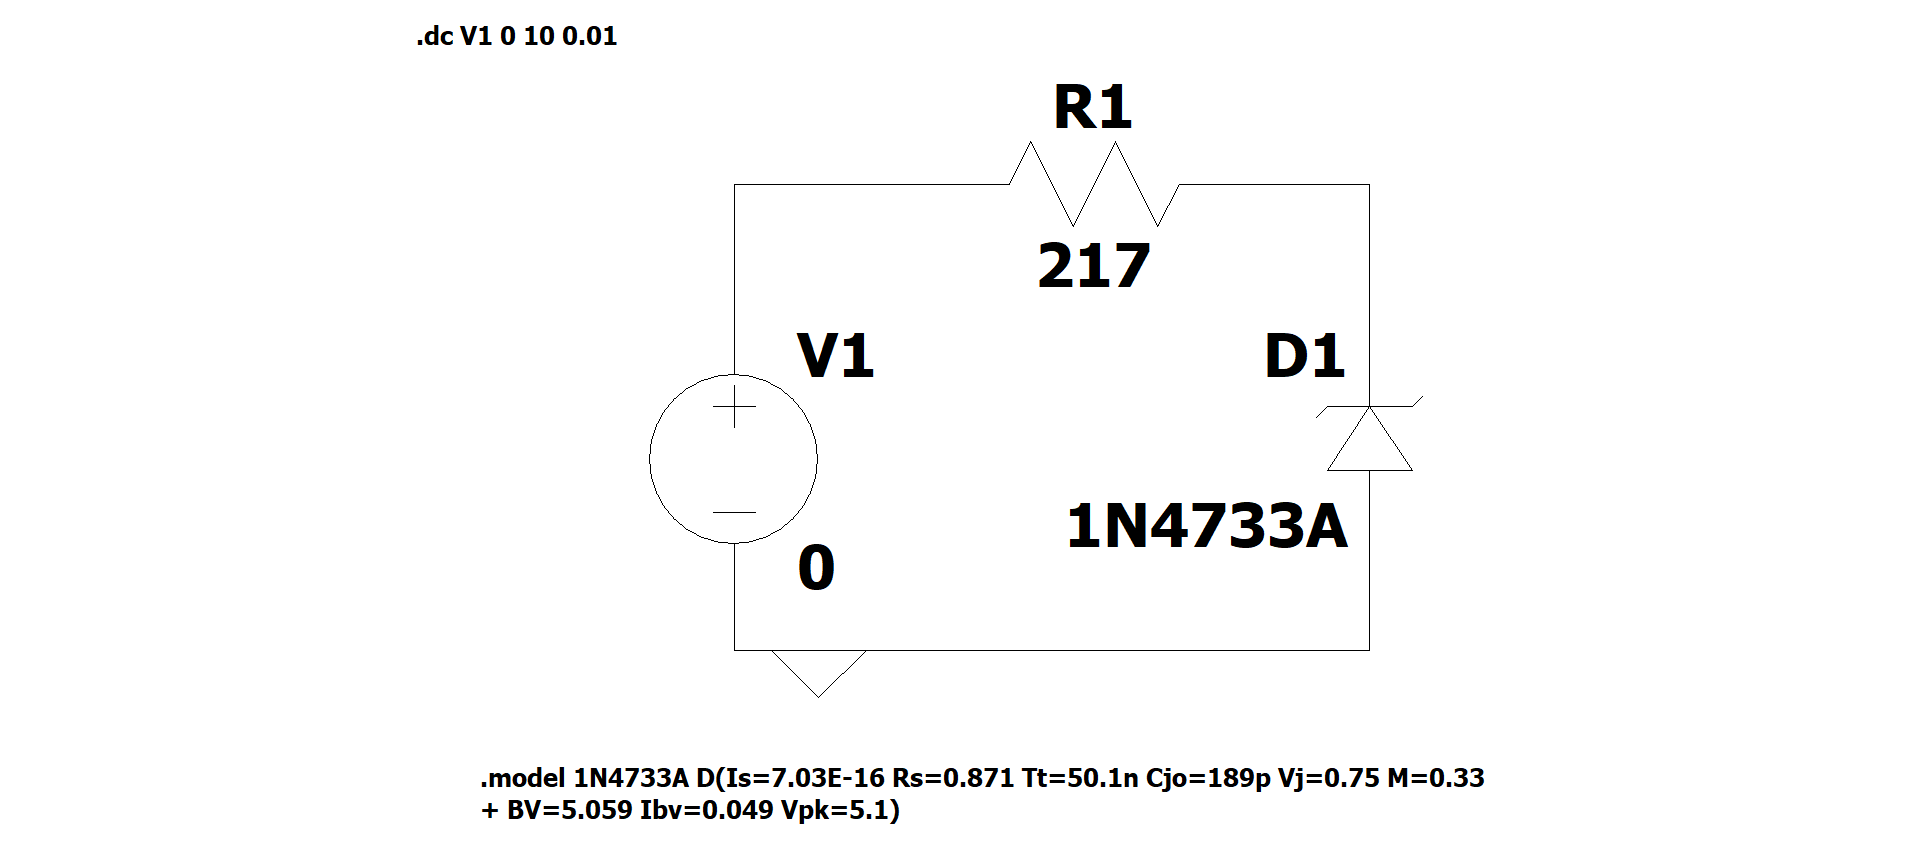
\includegraphics[width=\textwidth, height=4.5cm, keepaspectratio]{lab-06/assets/reverse-schematic.png}
    \caption{Schematic}
  \end{subfigure}
  \hfill
  \begin{subfigure}[b]{0.48\textwidth}
    \centering
    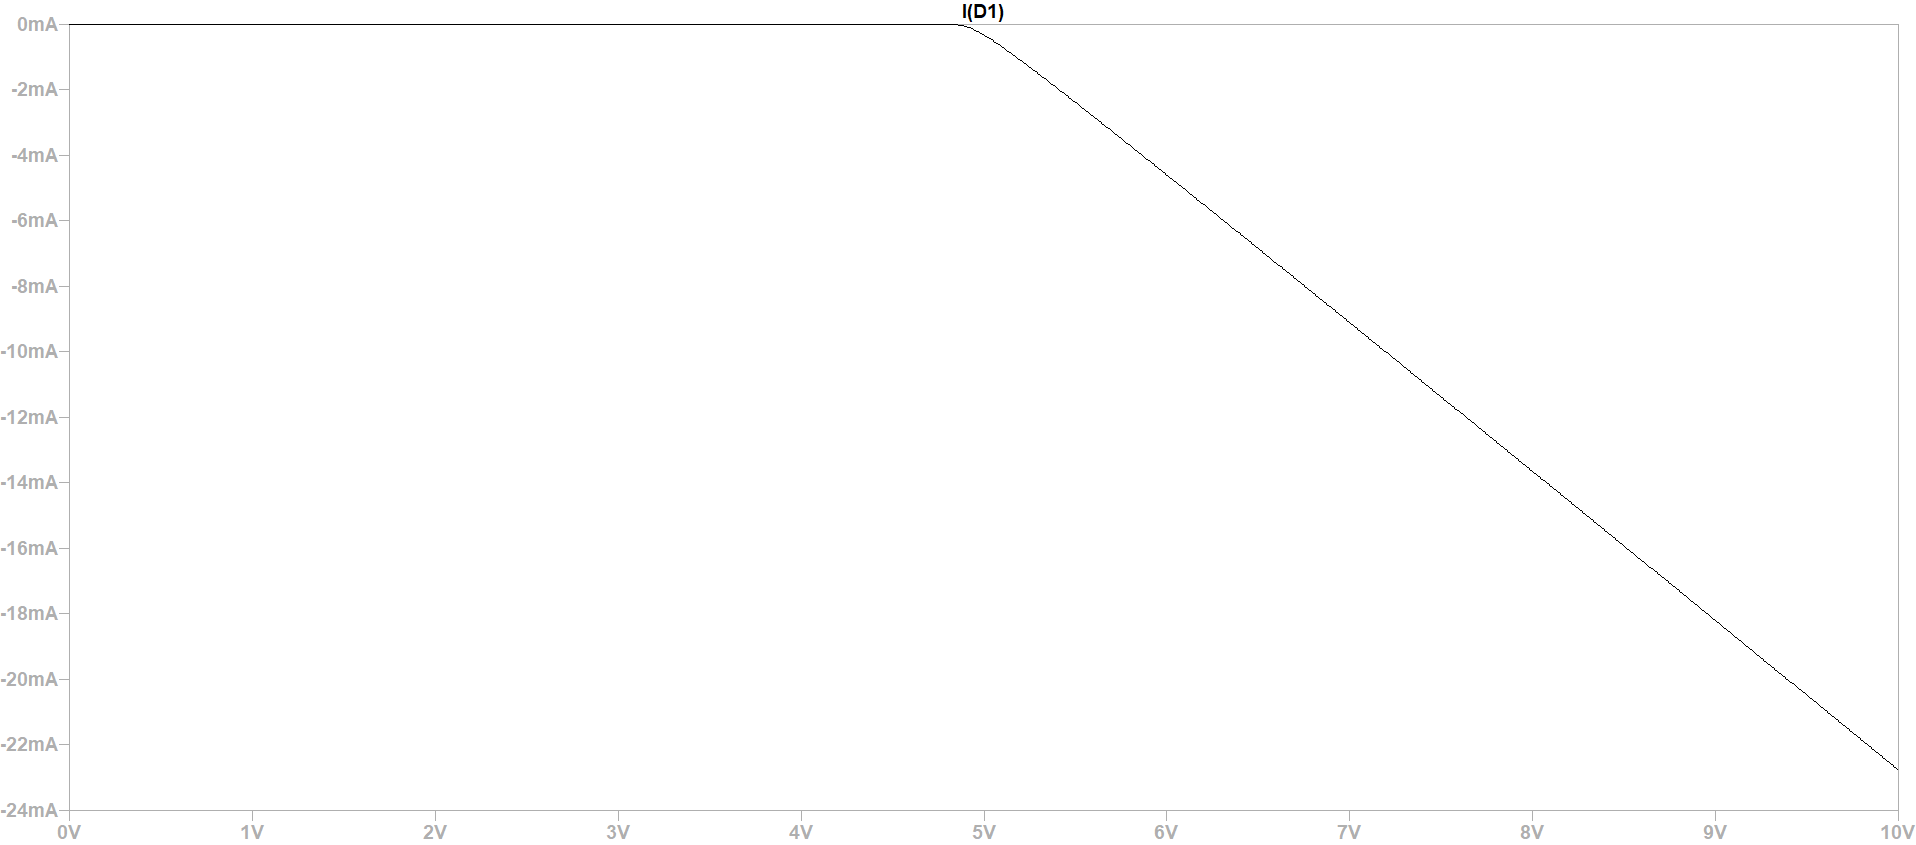
\includegraphics[width=\textwidth, height=4.5cm, keepaspectratio]{lab-06/assets/reverse-graph.png}
    \caption{Output}
  \end{subfigure}
  \caption{Simulation of Reverse Bias: (a) Schematic and (b) Output.}
  \label{fig:lab06_sim_reverse}
\end{figure}
